\documentclass{sig-alternate}[10pt]

% graphic declaration
\usepackage{graphicx}
\usepackage{listings}
\usepackage[english]{babel}
\usepackage{float}
\usepackage{color}
\usepackage{caption}
\usepackage{indentfirst}
\usepackage{amsmath}
\usepackage{fancybox}
\usepackage{algorithm}
\usepackage{algpseudocode}
\usepackage{multicol}
\usepackage{balance}
%\usepackage{svg}
\usepackage{pdfpages}

\definecolor{dkgreen}{rgb}{0,0.6,0}
\definecolor{gray}{rgb}{0.5,0.5,0.5}
\definecolor{mauve}{rgb}{0.58,0,0.82}

%\iffalse
%\lstset{frame=tb,
  %language=Java,
  %aboveskip=3mm,
  %belowskip=3mm,
  %showstringspaces=false,
  %columns=flexible,
  %basicstyle={\footnotesize\ttfamily},
  %numbers=none,
  %numberstyle=\tiny\color{gray},
  %keywordstyle=\color{blue},
  %commentstyle=\color{dkgreen},
  %stringstyle=\color{mauve},
  %breaklines=true,
  %breakatwhitespace=true,
  %tabsize=3
%}
%\fi

\lstset{%
  xleftmargin=0pt,
  belowcaptionskip=\bigskipamount,
  captionpos=b,
  escapeinside={*'}{'*},
  language=Java,
  tabsize=2,
  emphstyle={\bf},
  commentstyle=\it,
  stringstyle=\mdseries\ttfamily,
  showspaces=false,
  keywordstyle=\bfseries,
  morekeywords={then,end,String, Class, Object},
  columns=flexible,
  basicstyle=\scriptsize\ttfamily,
  showstringspaces=false,
  morecomment=[l]\%,
}

\graphicspath{ {data/} }

\begin{document}

\setcopyright{acmcopyright}
\conferenceinfo{MOBILESoft '16}{May 16--17, 2016, Austin, TX, USA}
\acmPrice{\$15.00}
%\doi{}

%
% paper title
% Titles are generally capitalized except for words such as a, an, and, as,
% at, but, by, for, in, nor, of, on, or, the, to and up, which are usually
% not capitalized unless they are the first or last word of the title.
% Linebreaks \\ can be used within to get better formatting as desired.
% Do not put math or special symbols in the title.
%\title{Expanding Limited Mobile Resources for Performance, Energy-Efficiency, and Privacy}
%\title{Extending Resource-Constrained Mobile Devices for Performance, Energy-Efficiency, and Privacy}
\title{Utilizing Nearby Distributed Computing Resources for Resource-Limited Mobile Devices}
%Resource-Constrained Mobile Devices}

%%%N-REX (Nearby-Remote Executor similar to T-Rex)

% author names and affiliations
% use a multiple column layout for up to three different
% affiliations
\numberofauthors{2}
\author{
\alignauthor Le Dinh Minh \\
\affaddr{Department of Computer Science} \\
\affaddr{Utah State University} \\
\email{minh.le@aggiemail.usu.edu}
\alignauthor Young-Woo Kwon \\
\affaddr{Department of Computer Science} \\
\affaddr{Utah State University} \\
\email{young.kwon@usu.edu}
}

% make the title area
\maketitle

\begin{abstract}
For the last decade, mobile devices have been significantly developed with powerful hardware facilities such as multicore CPUs, large and fast memory, fast network and high resolution displays. As a result, mobile applications deliver increasingly complex functionality from the recent past. Furthermore, rapid growth in application functionality requires ever greater hardware capability. Thus ensuring the quality of service in resources-limited execution environments remains a major challenge of mobile software development. To reduce execution time and save battery power, some functionality of mobile applications is often executed at a remote server. However, such an optimization mechanism (i.e., computational offloading) has only received much attention in the research literature due to difficult implementation, limited applicability, cost of the cloud, etc. In this paper, we present a novel distribution infrastructure that executes any functionality at a powerful remote server or nearby mobile devices using two distributed execution models---client/server and peer to peer. By means of a simple programming model, the programmer can easily adopt two distributed execution models in their applications. Our benchmarks and case studies demonstrate that the new distribution infrastructure can increase both performance and energy efficiency of mobile applications as well as introducing new feature (i.e., GPS, sensors) to the existing mobile devices.
\end{abstract}

\begin{CCSXML}
\begin{CCSXML}
<ccs2012>
<concept>
<concept_id>10010520.10010521.10010537.10010540</concept_id>
<concept_desc>Computer systems organization~Peer-to-peer architectures</concept_desc>
<concept_significance>500</concept_significance>
</concept>
<concept>
<concept_id>10010520.10010521.10010537.10003100</concept_id>
<concept_desc>Computer systems organization~Cloud computing</concept_desc>
<concept_significance>300</concept_significance>
</concept>
</ccs2012>
\end{CCSXML}
\ccsdesc[500]{Computer systems organization~Peer-to-peer architectures}
\ccsdesc[300]{Computer systems organization~Cloud computing}

\terms{Design}

\printccsdesc
\keywords{Mobile Computing, Remote Execution, Offloading, Peer to Peer, Runtime System}

\section{Introduction}
Mobile devices have been evolving at lightning pace with powerful hardware facilities such as multicore CPUs, large and fast memory, fast network and high resolution displays. Due to the significant development of mobile hardware, today's mobile applications are becoming more complex with a increasingly feature-rich nature. As a result, mobile devices often overtake the personal computer as a primary means of accessing computing resource. However, the resource demands (e.g., computation, memory, battery, etc.) of mobile applications often outstrip the hardware capacities of mobile devices. A particularly popular technique to extend limited mobile hardware is \emph{computational offloading}---executing CPU-intensive functionality at a powerful cloud-based server with the parameters and results transferred across a mobile network, thereby improving both performance and energy efficiency. 

Although computational offloading has been widely enjoyed in the research literature as an optimization mechanism that can utilize remote CPU resources, a majority of feature-rich mobile applications still suffer from resource constraints to provide quality user experiences. In addition, because computational offloading mechanisms have been developed by leveraging cloud computing technologies, in spite of their great advantages, the high operational cost of cloud infrastructures and the implementation difficulties of computational offloading have deterred programmers from actively applying computational offloading in their mobile applications. In particular, performance or energy benefits gained through computational offloading would be considerably low when comparing to the operational costs of cloud-based offloading server. Moreover, mobile devices can only executes computation-intensive functionality by accessing the CPU resources of the cloud-based server. Finally, implementing effective computational offloading optimizations often requires highly experienced programming skills and efforts \cite{kwon+:mobilesoft15}.

Nevertheless, computational offloading is still considered an important optimization mechanism for mobile applications as one of distributed execution models. Thus, in order to optimize mobile applications' executions and extend mobile devices' hardware capacity through distributed executions, we solve the following research problems: (1) how can mobile applications utilize remote computing resources at low cost? (2) how can the application programmer express the desired mobile hardware resources? (3) how can mobile devices allow using their resources without affecting the existing applications' executions? Solving these problems requires innovations in programming models and middleware design spaces. 

In this paper, we present a novel distributed execution model that not only optimizes mobile application's executions in terms of performance and energy efficiency, but also extends mobile device's hardware capability. In other words, mobile devices will be able to virtually add more hardware resources including computation, networking, memory, and sensors to the existing hardware setup. Our approach is realized as the following two major technical solutions: (1) a straight programming model that enables the programmer to write any execution task and (2) a runtime system that determines an execution strategy and distributes the requested execution task over the nearby or remote network. Our runtime system employs a dynamic, adaptive mechanism to determine the best distribution and execution strategy under different execution environments including diverse network conditions and heterogeneous mobile hardware capacity.

The experiments in 3 case studies have demonstrated the effectiveness of our approach, to extend limited mobile hardware resources, thereby improving performance and energy efficiency as well as bringing new hardware capabilities. By presenting our approach, this paper makes the following technical contributions:
\begin{itemize}
	\item \textbf{Simple programming model:} We provide simple APIs for programmers to easily deploy distributed mobile applications to take full advantage of external remote resources using our distributed execution model.
	\item \textbf{Lightweight runtime system:} Our runtime system efficiently distributes executions to available peers or offloading server, based on a peer selection algorithm. 	
	\item \textbf{A proof of concept infrastructure implementation:} Through three case studies, our system demonstrates how mobile hardware resources can be effectively shared.
\end{itemize}

%should go to the later part
%No internet connections are required, and it will help the owner to connect to the devices within a closed distance. By establishing connection between the two devices to form a pair, Wi-Fi Direct can provide the simple way to dynamically initiate a peer-to-peer network. Available on Android devices from version 4.0 (which more than 96\% of devices are using these days), as well as a number of Intel-featured laptops and game consoles, there is the high possibility of discovering the other mobile devices at anywhere.

%Job2P provides a simple and straightforward API interface to get rid of sophistication of network implementation, letting developers easily create their distributed mobile applications with capability of forming closed range network. In term of workload distribution, Job2P splits task and resource into the smaller units called jobs, and dispatch to the peers. To distributed jobs equitably among the peers, a decision making module is added to decide the amount of resource the peer has to handle bases on its percentage of availability. Moreover, our APIs can handle fault tolerant for network malfunctions.

The rest of this paper is structured as follows. Section \ref{sec:background} introduces a technological background for the main technologies used in this work. Section \ref{sec:approach} details our technical approach and Section \ref{sec:eval} discuss how we evaluated our approach. Section \ref{sec:related} compares our approach to the related state of the art. Section \ref{sec:conc} concludes this paper.
 
\section{Technical Background}
\label{sec:background}
In this section, we present the major technologies we used in this paper. The major technologies used in this work including computation offloading, remote execution, middleware, and WiFi direct. We will describe them in the following sub sections.

\subsection{Computational Offloading}   
Computation offloading has become a popular optimization technique for mobile applications \cite{maui,chun+:eurosys11,kwon+:icdcs12,wen2012energy}. It leverages the resources of cloud-based remote servers to execute portions of a mobile application's functionality. By executing some of the application's functionality in the cloud, offloading reduces the amount of energy consumed by the mobile device, thus saving its battery power. An additional benefit of computation offloading is improved performance efficiency, as cloud servers have hardware resource more powerful that those available on mobile devices. This technique is used as one of the distributed execution model in this paper.

\subsection{Remote Execution and Middleware}
Our approach uses features from mainstream middleware mechanisms for distributed execution as building blocks. Middleware systmes provide programming and runtime support to coordinates the execution of multiple remote processes. By eliminating the need for low-level network programming (e.g., managing sockets, marshaling/unmarshaling data, keeping track of processes) middleware systems offer convenient building blocks for constructing distributed systems. In our prior work \cite{kwon+:mobicase14-middleware}, we introduced a novel middleware architecture that optimizes performance and energy consumption by adapting various facets of middleware functionality dynamically in response to fluctuations in network conditions because network communication incurs high energy costs in mobile applications. The runtime system developed in this paper is derived from our prior middleware design.

\subsection{WiFi Direct}
The WiFi Direct \cite{alliance2010wi} is a new peer to peer standard built on top of the IEEE 802.11 to provide connections between WiFi devices without an Internet connection. Over a WiFi network, a WiFi device can discover any nearby WiFi devices without special configurations or setups. Once a connection is established, WiFi devices can communicate with each other as a client or an access point. WiFi Direct has been widely used to transfer content or share applications among mobile devices. Recently in Android, WiFi Direct has become available from Android 4.0 APIs. In this paper, our approach uses Android WiFi Direct \cite{wifi:p2p} to utilize nearby computing resources without any Internet connection or wireless access point. Even though the discovery operation of WiFi Direct is costly \cite{trifunovic2013slicing}, our approach is still efficient for heavy CPU-intensive executions or sharing hardware resources. 



%other name?
\section{Our Approach}
\label{sec:approach}
In this section, we present our approach, a distributed mobile execution model that can expand the resource capacities of mobile devices. We start by giving an overview of the approach and then describe its major parts.
 %Then, Section \ref{sec:eval} presents the experimental results of applying our approach to three case studies.

\begin{figure}
	\centering	
		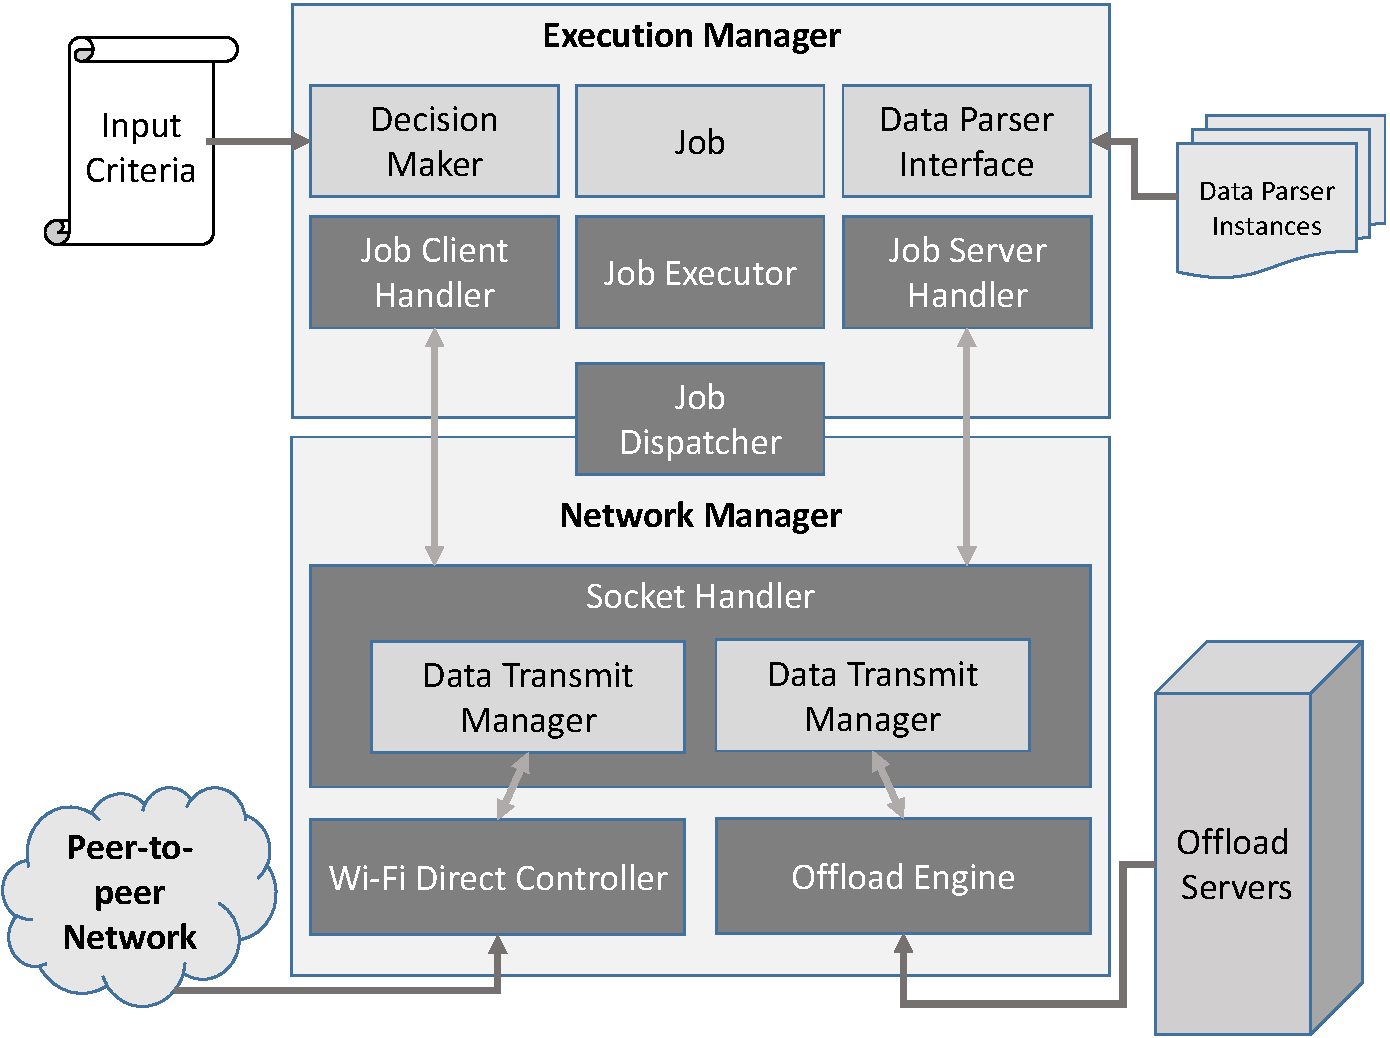
\includegraphics[width=.95\linewidth]{data/jobShareArch.pdf}	
	\caption{System architecture}
	\label{fig:architecture}
\end{figure}


\subsection{Approach Overview}
Figure \ref{fig:architecture} shows the overall system architecture, which main-ly consists of two parts: (1) \emph{WiFi Network Manager} (\emph{WNM}) discovers available mobile devices, checks the availability of the registered cloud-based remote servers, and then establishes a network connection for the data transmission; (2) \emph{Execution Handler} provides abstract functionality for job definition, execution and distribution. For the best execution result, \emph{Execution Handler} keeps track of current execution environments such as network conditions (e.g., delay, bandwidth) and system status (e.g., resource usage including CPU, memory). In addition, our important design choice is hiding the complexity of implementation details for application programmers. Thus, we offer a simple programming model that the programmer can easily import or extend. In the following discussion, we will discuss the details of the system architecture.

%It discovers available peers, establishes connections, and keeps track of the connections. 
\subsubsection{WiFi Network Manager}
To establish a network connection between nearby mobile devices over the WiFi network, we utilize the WiFi Direct technology. In particular, \texttt{WiFiDirectController} of \texttt{WNM} hides the complex WiFi Direct implementation details. As aforementioned in the previous section, to leverage computational offloading, the \texttt{OffloadEngine} module initiates a connection with our cloud-based offloading server when a WiFi access point (AP) is available \cite{kwon+:mobilesoft2015}, thus executing the job at a powerful remote server instead of looking for nearby devices. By providing transparent operations between the cloud-based server and nearby mobile devices, our approach separates a business logic from distributed execution models.

When an application starts, \texttt{WNM} calls \texttt{discoverPeers()} to search for available offloading servers registered in its configuration file. It also spreads acknowledgments to inform its availability to nearby mobile devices. If any offloading server or nearby devices receive a discovery message, its \texttt{WNM} module updates the new caller to its available device list, then simultaneously sends their information back to the caller in a JSON object (see \ref{ss_dfp}). Once all the devices are updated with the available device list, the network is organized as described in Figure \ref{fig:forming}. We provide the method \texttt{connectToADevice()} to make a connection with the best available mobile device. After establishing the connection, the mobile device starts to passively listen to job requests.

%invocation will be promoted as server and use the \texttt{ServerSocketHandler} to initiate server socket with an random port. If the invoked device is already a server, it will maintain its current state and continuously accept the new client. Moreover, since a device can either be a server to some peers, or serve as client to the others, this method is able to build up a close range peer-to-peer network.

Both \texttt{ClientSocketHandler} and \texttt{ServerSocketHandler} are constituted by a sub module named \texttt{DataTransmitManager}, which periodically observes input and output streams of parent socket (which can be either server or client socket) to verify checksum, check data consistency, send/receive data from the socket. Inheriting the \texttt{TransmitManager} abstract class, developer can instantiate their own version of \texttt{DataTransmitManager} to customize the data consistency checker or improve security. 

\begin{figure} 
	\centering
	\resizebox{0.5\textwidth}{!}{
		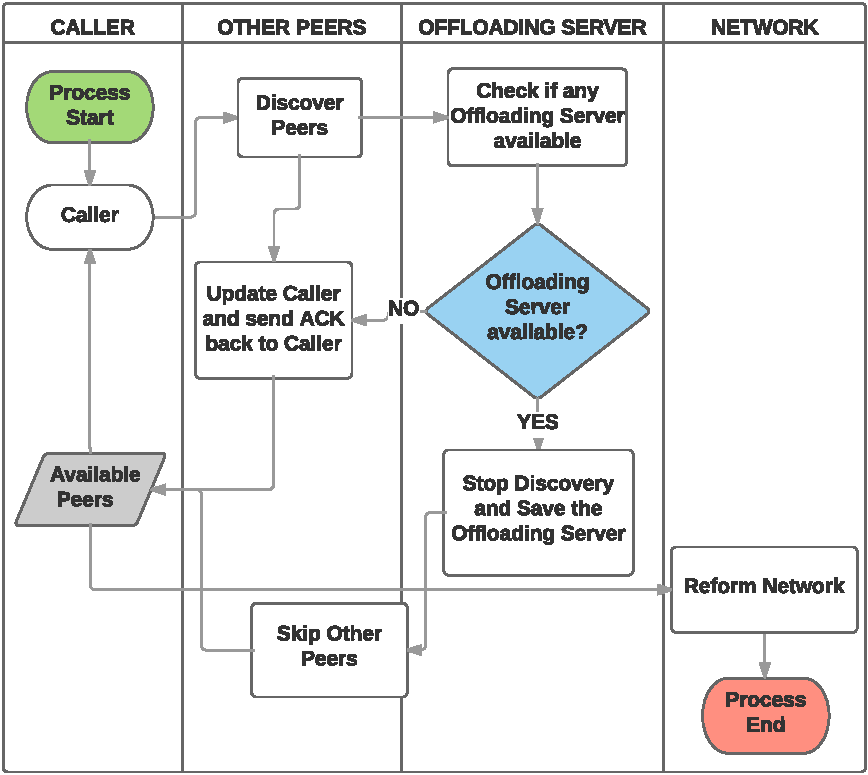
\includegraphics{data/discoverPeers.pdf}
	}
	\caption{Establishing a network connection between devices}
	\label{fig:forming}
\end{figure}


\subsubsection{Execution Handler}
\emph{Execution Handler} handles job definition, execution and distribution. \texttt{Job} (see \ref{prog_model}) is an executable unit defined by the programmer. By analyzing information of available mobile device list, \texttt{DecisionMaker} selects a number of highest responsibile devices and decides jobs with appropriate amount of conjunctional data. Then \texttt{JobDispatcher} dispatches them using \texttt{WNM} to the selected devices. On each remote device or offload server, \texttt{Job} and its partial data will be deserialized and executed by \texttt{JobExecutor} in synchronous mode. After that, the results will be return back to the caller by \texttt{JobClientHandler} and \text{JobServerHandler}. To facilitate adaptation with data heterogeneity, we define \texttt{DataParser} as a loosely coupled interface of \texttt{Job} to support determining mechanisms for: (1) serialization/deserialization object into binary format which is compatible for TCP transmission, (2) task partitioning, and (3) placeholder initialization and concatenation. To make the data type comprehensive to system in terms of reading, parsing or memory allocating, developer needs to supply instructions by instantiating an implementation of Data Parser for that type. 


\subsection{Programming Model} \label{prog_model}
Our system has a simple programming model that enables the programmer to easily implement remote functions. As described in Listing \ref{code:job_def}, we provide a \texttt{Job} abstract class that will be extended by the programmer to specify which functionality should be executed remotely. Also, to support dynamic class loading in Dalvik VM, we provide the \texttt{DexCreator} commandline tool that compiles the \texttt{Job} Java class file into a Dex package. The Dex package and sliced resources are packed as a \texttt{JobData} object by \texttt{JobDispatcher} and then dispatched to the available mobile devices or the cloud-based server. Next, the recipient of the \texttt{JobData} checks a checksum field to confirm the consistency, and then deserializes the object into \texttt{Job} and resources for the execution.

\begin{figure}
\noindent \shadowbox{%
\begin{minipage}{240pt}
	\begin{lstlisting}
	public abstract class Job {
	  public abstract Object exec(Object param); }
	\end{lstlisting}	
\end{minipage}}	
\noindent \shadowbox{%
\begin{minipage}{237pt}
  \begin{lstlisting}
public interface DataParser {  
  public Class getDataClass();
  public byte[] parseObjectToBytes(dataObject);
  public Object parseBytesToObject(byteArray);
  public Object getSinglePart(..., 
		numOfParts, sOffset, eOffset);    
  public Object createPlaceholder(jsonMetadata);
  public Object copyPartToPlaceholder(... 
					partDataObject, sOffset, eOffset);
  public void destroy(dataObject);  }
  \end{lstlisting}	
\end{minipage}
}	
\captionof{lstlisting}{Provided APIs (top: Job, bottom: DataParser)}
\label{code:job_def}
\end{figure}


\subsubsection{Data Parser} \label{data_parser}
The code snippet in Listing \ref{code:job_def} shows the important methods of \texttt{DataParser} that user needs to implement. The \texttt{DataParser} interface has the following methods:
\begin{itemize}
	\item \texttt{getDataClass()} returns data type.
	\item \texttt{parseObjectToBytes(object)} instructs system to serialize an object to binary array. In Android, not every object can be serialized, for instance, Bitmap.  
	\item \texttt{parseBytesToObject(byte[])} deserializes a binary array back to object.
	\item \texttt{getSinglePart()} returns a data slide based on number of parts (\texttt{numOfParts}) and its \texttt{index}. Code snippet (\ref{code:get_single_part}) shows an example getting one slice from a bitmap by \texttt{index}. When app runs, \texttt{JobDispatcher} will use this method to partition the task into slices.
	\item \texttt{copyPartToPlaceholder()} instructs the application to merge it to the placeholder when a result is partially retrieved from a distant peer.
\end{itemize}

In our case studies (see Section \ref{sec:eval}), we implemented three default parsers for bitmap images, text, and GPS, respectively. 

\subsection{Runtime System} \label{scheduling}
Once a peer-to-peer network is constructed by our system, each peer participating in the network can distribute jobs to other peers. Specifically, before making a remote job execution, \texttt{DecisionMaker} determines available peers in accordance with the level of available resources by inquiring peers' status via an \texttt{IRS} message. Once one receives the IRS request, its \texttt{DecisionMaker} immediately responds to the request with the capability information of CPU, memory and battery usage at that time depicted in Figure \ref{fig:forming}.

%\begin{figure}
%\centerline {
%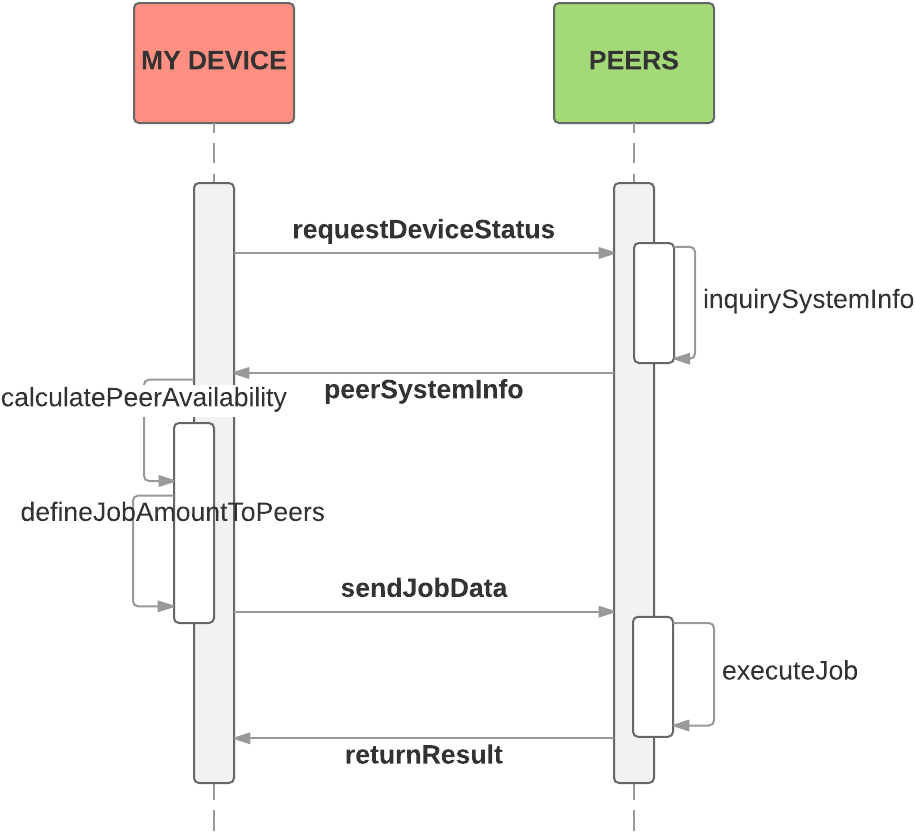
\includegraphics[width=0.45\textwidth, natwidth=915, natheight=837]{data/checkStatusFlow}
%}
%\caption{Workflow between mobile devices.}
%\label{fig:checkStatus}
%\end{figure}

\subsubsection{Finding available devices}\label{ss_dfp}

A mobile device at any time maintains a certain number of connections with the others. Before delivering jobs, it dispatches IRS messages to all the peers for acknowledgment of their availability ($RL$ - Level of Responsibility). If a peer receives an IRS, its \texttt{DecisionMaker} will capture its configuration and corresponding usage states to generate a response in JSON format, The code snippet (\ref{code:jsonResponse}) shows such a typical response.\\

\begin{figure}
\noindent \shadowbox{
\begin{minipage}{240pt}
\begin{lstlisting}
JSON : DeviceInfo {
  "device": "LG-Volt", 
	"RL": 24.83,
  "availability": "off", 
	"network": "low", 
	"gps": "on",	
  "cpu": {"usage": "0.3", "speed": "1.3", "cores": 4},
  "memory": {"usage": "0.5", "total": 2},
  "battery": {"usage": 0.85, "total": 2800}}
\end{lstlisting}			
\end{minipage}}	\\
\noindent \shadowbox{%
\begin{minipage}{243pt}	
\begin{lstlisting}
JSON : Condition {"RL": "max", "gps": "on"}
\end{lstlisting}\end{minipage}}	

\captionof{lstlisting}{A JSON response format and initiative condition.}
\label{code:jsonResponse}

\end{figure}

Where \texttt{device} parameter can be either device name (if it is device) or \texttt{server host/IP} (if it is offloading server), $RL$ is the device's Level of Responsibility (for estimation of $RL$ and the other parameters, see \ref{ss_jqfp}), \texttt{availability} indicates whether the device is feasible for handling job. \texttt{network} gives the network status, which can be either \texttt{high}, \texttt{low} or \texttt{off} (no connections), and \texttt{gps} is information of GPS being \texttt{on} or \texttt{off}. Finally \texttt{cpu}, \texttt{memory} and \texttt{battery} are the status of the essential resources at the time of response. 

In any IRS response, \texttt{availability} is determined by the remote device which value can be assigned to \texttt{on} or \texttt{off}. The \texttt{off} value informs the caller that it is not available due to temporary shortage of resource and therefore prevents the caller from sending jobs. Only the devices with \texttt{availability} set to \texttt{on} will accept jobs for execution. The value is given based on whether the device has bypassed the threshold of battery usage which is by default set to 0.8 (or 80\% overall usage). User can override those thresholds by updating the \texttt{availability-thresholds} in the configuration file before app initialization. 

In the above example (code snippet \ref{code:jsonResponse}), the battery usage is 0.85 or 15\% remaining, so the \texttt{DecisionMaker} on it states that its \texttt{availability} is \texttt{off} and it won't be able to handle any jobs.

To make the system adjustable to wide range of resource usages with regard to energy and performance efficiency, the IRS criteria (Example in \ref{code:jsonResponse}) is added to the app configuration so that the \texttt{DecisionMaker} can check it by going through 3 following steps
\begin{itemize}
	\item \emph{If $RL$ is max}: Select one device having max $RL$ and match the other criteria, then finish.
	\item \emph{If offloading server available}: Select the first available server, then finish.
	\item \emph{If other criteria are matched}: Select a list of available devices having matched conditions.
\end{itemize}
Algorithm \ref{alg:select_peers} describes in detail the three above steps.

\begin{algorithm}

\caption{Selecting available peers}
\label{alg:select_peers}
\begin{algorithmic}[1] 
\begin{scriptsize}
\Function{selectPeers()}{}
\State Send IRS requests to all peers 
\State $CriteriaList \leftarrow IRSCriteria$
\State $P_{AV} \leftarrow HashMap(DeviceId, P)$

\If {$CriteriaList.RL = max$}
  \ForAll{$Resp_{IRS}$ in \{Incoming IRS Responses\}}
  	\State Find max $RL$ with other criteria in $CriteriaList$
		\State Assign device with max $RL$ to $P_{AV}$
  	\State \Return $P_{AV}$
  \EndFor
\EndIf

\ForAll{$Resp_{IRS}$ in \{Incoming IRS Responses\}}
  \If {$Resp_{IRS}[device] = server$}
  	\State Reset $P_{AV}$ 
  	\State $P_{Info} \leftarrow WiFiDevices.get(DeviceId)$
  	\State $P_{AV}[DeviceId] \leftarrow P_{Info}$
  	\State \Return $P_{AV}$
  \EndIf

  \If {All condition statements are satisfied} 
  	\State $P_{Info} \leftarrow WiFiDevices.get(DeviceId) + $
		\State
			\hspace{\algorithmicindent}
			\hspace{\algorithmicindent}
			\hspace{\algorithmicindent}
			\hspace{\algorithmicindent}
			$Resp_{IRS}[RL]$
  	\State $P_{AV}[DeviceId] \leftarrow P_{Info}$
  \EndIf
\EndFor

\State \Return $P_{AV}$
\EndFunction
\end{scriptsize}
\end{algorithmic}

\end{algorithm}

Algorithm \ref{alg:select_peers} explains how the caller selects appropriate peers from its connection list. Specifically, $P_{AV}$ stands for map of available peers and $WiFiDevices$ is the device information list.\\

\subsubsection{Job quantitation for peers}\label{ss_jqfp}
To assign a job to multiple peers, the runtime system collects the available resource information from each mobile device. Specifically, the percentage of CPU usage is calculated using the \texttt{/proc/stat} system file as follows:
\begin{equation}
\label{eq:cpu_usage}
Usage_{CPU} = \frac{(\sum{T_{CPU2}} - T_{Idle2}) - (\sum{T_{CPU1}} - T_{Idle1})}{(\sum{T_{CPU2}} - \sum{T_{CPU1}})}
\end{equation}

\noindent where $\sum{T_{CPU}}$ is total active time and $T_{Idle}$ is idle time. For the memory usage, $Usage_{Mem}$ is calculated by accessing \texttt{MemoryInfo} of Android APIs such as $Mem_{Avail}$ and $Mem_{Total}$. Finally, we  calculate the battery usage, $Usage_{Batt}$. Next, to determine the appropriate amount of data to each mobile device, we introduce $RL$ parameter as follows:
\begin{equation}
\label{eq:res_level}
%\begin{\footnotesize}
RL = \frac{N_{Cores} \times CPU_{Speed}}{Usage_{CPU}} + \frac{Mem_{Spec}}{Usage_{Mem}} + \frac{Batt_{Spec}}{Usage_{Batt} \times 1000}
%\end{\footnotesize}
\end{equation}

\noindent where $RL$ is an indicator to the level of availability of mobile devices. The smaller $RL$ means the higher availability. $N_{Cores}$ is the number of CPU cores. $CPU_{Speed}$ is speed of single core in GHz. $Mem_{Spec}$ is the memory capacity in GB and $Batt_{Spec}$ is the battery capacity in uAh. For example, if $Usage_{CPU}$ is 0.3, $Usage_{Mem}$ is 0.5 (i.e., half of 1GB memory has been consumed), and $Usage_{Batt}$ is 0.7 or 70\% used over a 2800uAh capacity battery, then $RL$ will be $$RL = \frac{5.2}{0.3} + \frac{1}{0.5} + \frac{2800}{0.7 \times 1000} = 23.33$$

If the selected peer is a powerful cloud-based server, $Batt_{Spec}$ is considered $\infty$ and $Usage_{Batt}$ is 0. According to Equation \ref{eq:res_level}, $RL$ will also be $\infty$. To make the calculation simple, we assign the maximum value of Integer to $RL$. To reduce the calculation overhead on the calling side, $RL$ is prematurely calculated on each peer and then sent to the caller in response to the IRS request.

Finally, the \texttt{DecisionMaker} assigns the job with the appropriate amount of data ($M_{i}$) in accordance with the following equation:
\begin{equation} 
\label{eq:data_amount}
M_{i} = M\frac{RL_{i}}{\sum_{j = \overline{1,n}}{RL_{j}}}
\end{equation}

\noindent where $M$ is total size of data in bytes. $n$ is the number of mobile devices, where $i$-device has responsibility level $RL_{i}$. It is obvious that in the network with an offloading server, $M_{offload}$ is almost equal to $M$, and thus we can flush the full task with heavy computation to the offloading server. Algorithm \ref{alg:assign_job} describes how \texttt{DecisionMaker} assign a job appropriately while considering the availability of each mobile device. The algorithm returns the amount of data in binary length with two offsets that indicate the location of the data.

\begin{algorithm}
\caption{Assigning a job}
\label{alg:assign_job}
\begin{algorithmic}[1]
\begin{scriptsize}
\Function{assignJobs()}{}
\State $M \leftarrow {getDataSize()}$
\State $RL_{Total} \leftarrow 0$ 
\For {$P$ in \{$P_{AV}$\}}
  \State $RL_{Total} \leftarrow RL_{Total} + P[RL]$
\EndFor
\\
\State $firstOffset, lastOffset \leftarrow 0$
\State $jobData \leftarrow Null$
\State $job \leftarrow {readJobFile()}$
\State $M_{C} \leftarrow 0$
\\
\For {$i = 1$ to $P_{AV}.length$}\\
  \State $M_{i} \leftarrow M\frac{RL_{i}}{RL_{Total}}$\\
  \State $firstOffset \leftarrow M_{C} $
  \State $lastOffset \leftarrow M_{C} + M_{i}$
  \State $jobData \leftarrow DataParser.getSinglePart($
  \State 
		\hspace{\algorithmicindent}
		\hspace{\algorithmicindent}
		\hspace{\algorithmicindent}
		\hspace{\algorithmicindent}
		\hspace{\algorithmicindent}
						$firstOffset, lastOffset)$
  \State $dispatchJob(\{job, jobData\})$\\
  \State $M_{C} \leftarrow lastOffset$
  
\EndFor

\EndFunction
\end{scriptsize}
\end{algorithmic}
\end{algorithm}

\subsection{Estimating Energy Consumption}
As compared to estimating the energy consumption in cellular networks, in a WiFi network the energy consumption can be easily estimated. The total energy consumption can be calculated as follows:
$$E_{0} = E + E_{w}$$
\noindent where $E_{w}$ is the energy that the app requires for waiting. Then, we calculate the energy consumed by sending a job to other peers through the WiFi Direct technology as follows:
$$E_{p2p} = E(\frac{RL_{0}}{\sum_{i = 1}^{n}{RL_{i}}}) + E_{WiFi} + E_{w}$$ 
\noindent $n$ is the number of devices. $RL_{i} (i = \overline{1,n})$ is the responsibility level of each mobile device. 

However, we do not consider $E_{w}$ because it will depend on the appearance of applications. For example, if an application has no GUI, $E_{w}$ will cause very little effect. From the two above equations, we can calculate the energy consumption differences between two job processing mechanisms:
$$E_{Diff} = E_{0} - E_{p2p}$$ 
or 
\begin{equation}
\label{eq:energy_diff}
E_{Diff} = E(1 - \frac{RL_{0}}{\sum_{i=1}^{n}{RL_{i}}}) - E_{WiFi}
\end{equation}

Since WiFi is known to drain a battery linearly by time during transmission \cite{wifi_energy}, particularly it can be represented by $y = 17.01x - 0.93$ for downloading and $y = 17.31x - 2.28$ for uploading, where $y$ stands for percentage of battery consumed when using Wi-Fi for a period of $x$ hours. Therefore, under non-adventitious circumstances, equation (\ref{eq:energy_diff}) infers that in a mobile system with a certain number of devices in different levels of responsibility, if E is big enough, or in other words, if the task to perform is big enough, then $E_{Diff} > 0$ will result in, thus deploying a peer-to-peer cluster will give a great benefit in terms of energy efficiency. The bigger value of $E_{Diff}$, the more benefit we will gain. 

In addition, if a cloud-based offloading server is available in the network, $RL$ and $E_{Diff}$ are calculated as follows: $\sum_{i=1}^{n}{RL_{i}} \rightarrow \infty$, $E_{Diff} = E - E_{WiFi}$ which is the maximum value under the same conditions.

\subsection{API Usage Scenario}
The programming model should be simple, so that application programmers can integrate with a few steps. This section will describe step-by-step the way to utilize our API to enable a typical peer-to-peer network.

\subsubsection{Defining a Job}
Job implementation is the prerequisite work to determine what to execute on the remote device and how to cast and manipulate data from the abstract object. According to section \ref{prog_model}, a developer needs to implement the Job class file separately by overriding the \texttt{exec()} method and casting the abstract input parameter to the concrete one. Then run the \texttt{DexCreator} tool on the Job class to compile and compact it into the DEX jar package. The final outcome is the \texttt{job.jar} file, which should be saved in the internal storage of the caller device. In order to simplify, we can store it in the \texttt{Download} folder.  

\subsubsection{Implementing an Application Using APIs}
This section describes three basic steps to implement an Android application to utilize our APIs

\textbf{\emph{Message Handler:}}
The Message Handler is required to be instantiated at the beginning. In particular, an instance of \texttt{UIHandler} is initiated to receive messages from system when it goes into runtime. While the system is in progress, the log and information messages will periodically be returned with label \texttt{MAIN\_INFO} (Code snippet \ref{ui_handler}). When each job result comes, \texttt{ExecutionHandler} will collect and handle by partially put into a placeholder. When all results have arrived, the placeholder with label \texttt{MAIN\_JOB\_DONE} will be returned to inform the completion of job collaboration, as well as bringing the final result back to the main app UI.

\begin{figure}
\noindent \shadowbox{%
\begin{minipage}{239pt}	
	\begin{lstlisting}
Handler mainUiHandler = new Handler() {
	public void handleMessage(Message msg) {
		switch (msg.what) {
			case Utils.MAIN_JOB_DONE: { ... }
			case Utils.MAIN_INFO: { ... } }	} };
	\end{lstlisting}
\end{minipage}
}
\captionof{lstlisting}{UI handler}
\label{ui_handler}
\end{figure}

\textbf{\emph{Data Parser:}}
Secondly, the developer needs to declare \texttt{DataParser} to determine the data-type and the relevant parser to equip the system for manipulating data at run-time (see sub section \ref{data_parser}). \texttt{ExecutionHandler} is the main component which wraps up the complexity, and exposes only the necessary functions like \texttt{discoverPeers()} and \texttt{dispatchJob()}. To send ACK messages to other peers for exchanging acknowledgments and reforming network, we need to call \texttt{discoverPeers()} function on the program, which should be done as soon as the application starts.

\begin{figure}
\noindent \shadowbox{%
\begin{minipage}{245pt}
  \begin{lstlisting}
public Object getSinglePart(object, sOffset, eOffset) {
  Bitmap bmpData = (Bitmap) data;
  int pWidth = eOffset - sOffset;
  return Bitmap.createBitmap(bmpData, sOffset, 
									0, pWidth, bmpData.getHeight()); }
  \end{lstlisting}	
\end{minipage}}	
  \captionof{lstlisting}{Example of \texttt{getSinglePart()} for Bitmap}
  \label{code:get_single_part}

\end{figure}

\textbf{\emph{Discovery Peer and Dispatching Jobs}}

When the network is formed and connections are held with some other peers, \texttt{dispatchJob()} will be called to locate the resources and the job which is predefined in local storage, it then invokes \texttt{DecisionMaker} (sub section \ref{scheduling}) for job splitting and binary serialization. Finally jobs will be dispatched over the socket.

\begin{figure}
\noindent \shadowbox{%
\begin{minipage}{245pt}
	\begin{lstlisting}
dataParser = new BitmapJobDataParser();
jobHandler = new JobHandler(this, dataParser);

jobHandler.setSocketListener(
	new JobHandler.JobSocketListener() {
		@Override
		public void socketUpdated(... isConnected){
			...
		}});
deviceList.setAdapter(jobHandler.getDeviceListAdapter());
jobHandler.discoverPeers();

String dataPath = downloadPath + "/mars.jpg";
String jobPath = downloadPath + "/Job.jar";
jobHandler.dispatchJob(dataPath, jobPath);
\end{lstlisting}
\end{minipage}}

\captionof{lstlisting}{Using DataParser and JobHandler}
\end{figure}

\section{Evaluation}
\label{sec:eval}
This section describes the micro benchmarks and case studies that evaluate the effectiveness of our approach. The experimental setup includes a testbed with 5 Android phones. Table \ref{table:devices} shows the device-specific values.

\begin{table}[h]
\caption{Specifications of our test devices}
\label{table:devices}
\centering
\begin{tabular}{| l | l | l | l |}
    \hline
    Phone & CPU & RAM & Battery \\ \hline
    LG Volt & Quad-core 1.2GHz & 1GB & 3000mAh\\ \hline
		LG Opt. GK & Quad-core 1.7GHz & 2GB & 3100mAh\\ \hline
		LG G Stylo & Quad-core 1.2GHz & 1GB & 3000mAh\\ \hline
		LG Tribute & Quad-core 1.2GHz & 1GB & 2100mAh\\ \hline
		Galaxy S5 & Quad-core 2.5GHz & 2GB & 2800mAh\\ \hline
\end{tabular}
\end{table}

\subsection{Micro Benchmark}
We started the evaluation with micro benchmarking energy consumption of the system when mobile devices maintain connections in idle state, to figure out the cost of network maintenance overhead. Using Monsoon Power Monitor device \cite{moosoon} to replace battery and measure on one caller, we evaluated overhead based on accumulation of energy consumption by time. The Figure (\ref{fig:microb_24}) shows the outcome of the caller measuring from 0 to 100 seconds when preserving connections with 1, 2 and 3 other peers. 

\begin{figure}
	\hspace*{-0.15cm}
	\resizebox{0.5\textwidth}{!}{
		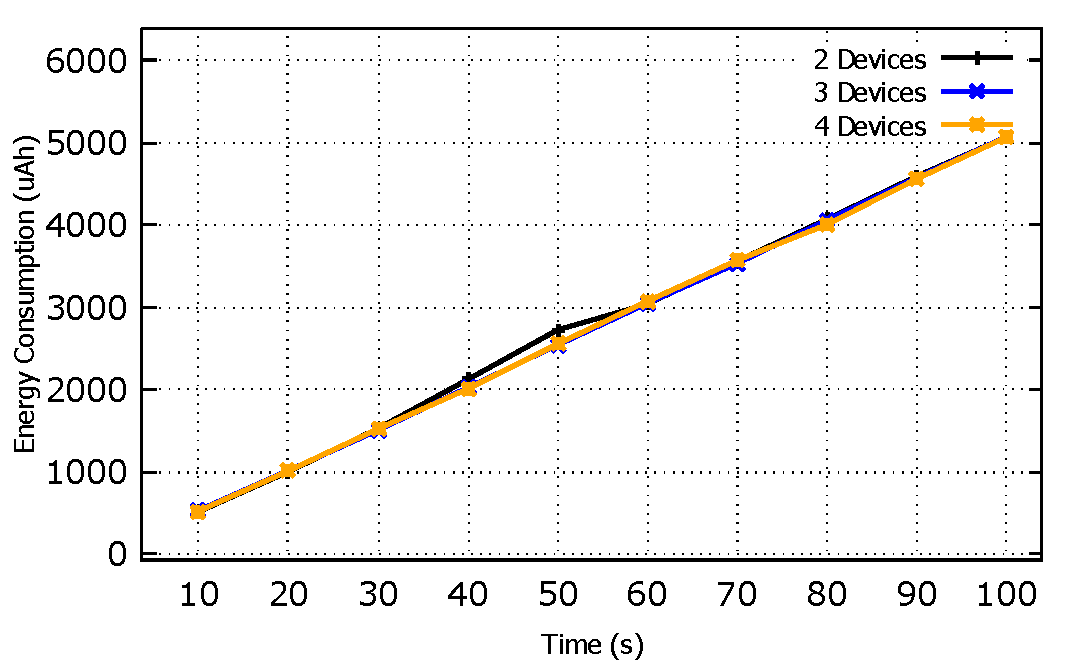
\includegraphics{data/ovh.pdf}
	}
	\caption{Energy consumption cumulation on caller in multi-device clusters}
	\label{fig:microb_24}
\end{figure}

According to the figure \ref{fig:microb_24}, it is revealed that in idle condition without transmitting any data, the energy consuming variability on each device within the P2P network is linear and mostly identical at any time, regardless of the number of devices to which it connects. This result is completely harmonized with results from \cite{wifi_energy}, especially since we transmit the same amount of data regularly over Wi-Fi connection. From the statistic information we collected, the energy variability of one device within P2P network in idle condition can be represented by the below linear formula

\begin{equation}
\label{eq:wifi_overload}
E_{WiFi} = t \times 50
\end{equation}

Where $t$ is accumulated time in milliseconds and $E_{WiFi}$ is energy used by system in uAh (micro ampere hour).

\subsection{Case Study}
To measure the performance of the system equipped with our APIs, we decorated a small testbed with collaboration of 5 different Android devices to perform our 3 test cases:
\begin{itemize}
	\item \textbf{Image Processing:} In this case study, we initiated a P2P network to blur a large size image, which could not be loaded and processed on a any single mobile device due to the limited memory space in mobile devices. Then, we distributed the blurring job to 1 to 4 mobile devices. 
	%Particularly, to process an image with size $4000 \times 4000$ and 4 bytes to express each pixel color, application must spare the amount of memory equivalent to 64MB which is way too much for a device, which occasionally returns out of memory exception.
	\item \textbf{Internet Access:} In this scenario, we defined an Internet access request for a mobile device that has limited network connection or no Internet connection, so that mobile applications could download remote data.
	\item \textbf{GPS Sharing:} Because establishing a GPS connection is a highly energy-intensive operation, it would be impossible for a device with low battery to frequently update its location information. We built a simple application that can benefit GPS locations from healthier devices. In addition, our system can be used for Internet of Things devices that do not have GPS sensors.
\end{itemize}

\subsection{Case Study Implementations}

\subsubsection{Image Processing}
We applied blur effect, one of the high energy consuming image processes. We run the test repeatedly on two image inputs, the first image has size $2500 \times 1405$ and the second size is $4326 \times 2856$. For the second image, with 4 bytes allocated for each pixel, device had to allocate around $50MB$ of heap to open and hold another $50MB$ for the result, thus leading to app crash all the time. This problem will only be solved with the help of other collaborative peers to solve overload in terms of memory and energy consumption.

\textbf{\emph{Design:}}
The most important part when applying APIs for image processing is defining the \texttt{DataParser} (see code snippet (\ref{code:job_def})) for Bitmap with a divide strategy in vertical cut. For an input image, the \texttt{firstOffset} and \texttt{lastOffset} will decide the first and last offsets of the vertical cut correspondingly throughout the width, from the top to the bottom edges. The algorithm of the vertical cut is described in the code snippet (\ref{code:get_single_part}). Regarding the placeholder, we override the \texttt{getJsonMetadata()} method to return a simple JSON string like below:

%\noindent \shadowbox{%
%\begin{minipage}{245pt}
	%\captionof{lstlisting}{JSON for initiating placeholder}
	\begin{lstlisting} 
	JSON { "width": 4326, "height": 2856 } 
	\end{lstlisting}
%\end{minipage}
%}

The method \texttt{createPlaceholder()} will parse this JSON object to obtain \texttt{width} and \texttt{height} as the inputs to initiate an empty placeholder bitmap. Finally \texttt{copyPartToPlaceholder()} method will place the partial result bitmap into its correct location on the placeholder defined by \texttt{sOffset} and \texttt{eOffset}.\\

\begin{figure}
\noindent \shadowbox{%
\begin{minipage}{245pt}
	\begin{lstlisting}
public Object copyPartToPlaceholder(placeholder, 
										part, sOffset, eOffset){
	Bitmap bmpPart = BitmapFactory.decodeByteArray(part...);
	int pieceWidth = partBmp.getWidth();
	Canvas canvas = new Canvas(placeholder);
	canvas.drawBitmap(bmpPart, sOffset, 0...);
	return null;
}
	\end{lstlisting}
\end{minipage}}
	\captionof{lstlisting}{Merging the result}
\end{figure}

When all the partial bitmaps are received, the system throws a message titled \texttt{MAIN\_JOB\_DONE} to the UI in which \texttt{msg.obj} contains the final bitmap.

\begin{figure*}
	\centering
	%\resizebox{0.39\textwidth}{!}{
	%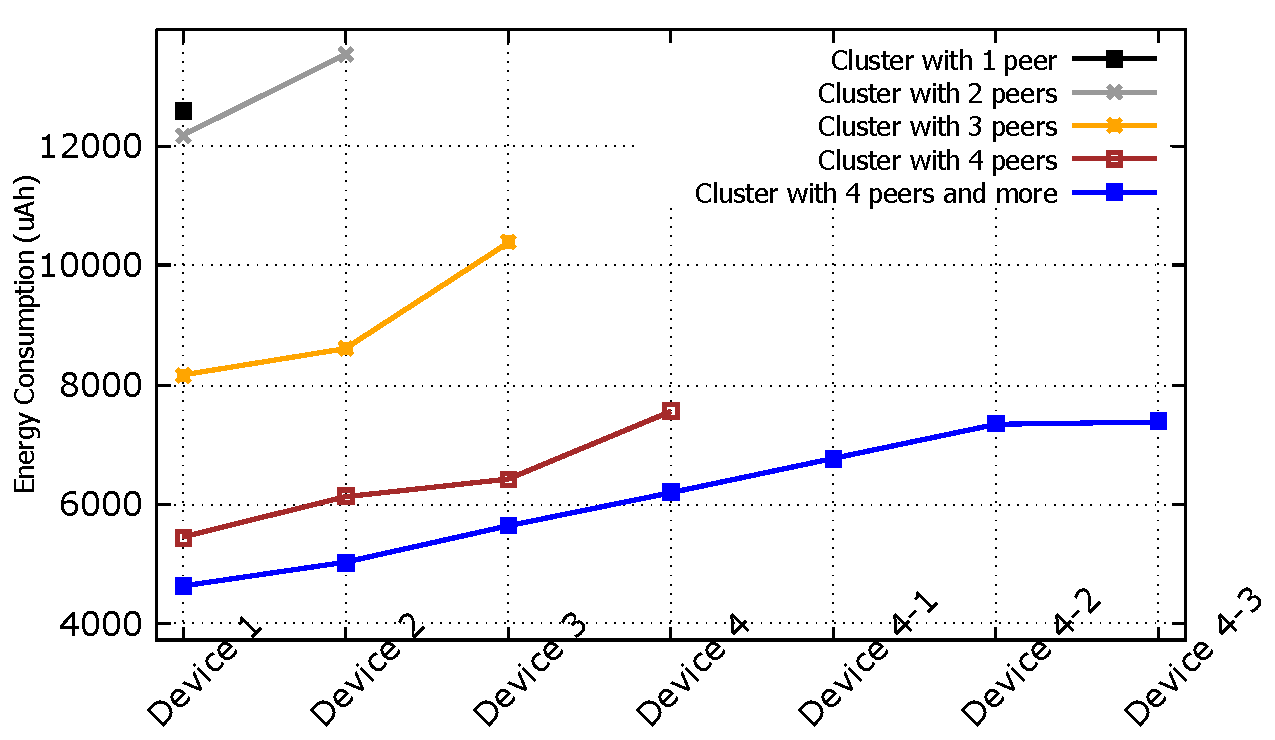
\includegraphics[width=0.32\textwidth]{data/img_large_perf_full.pdf}
		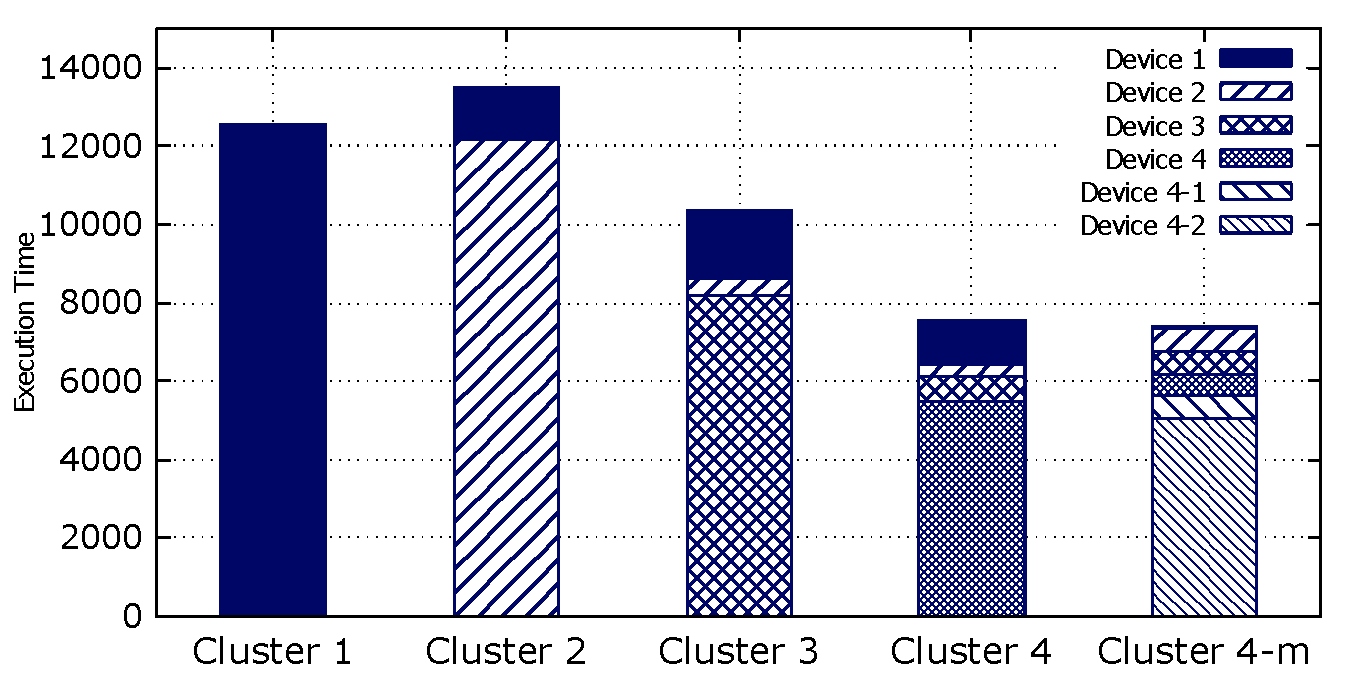
\includegraphics[width=0.39\textwidth]{data/img_perf.pdf}
		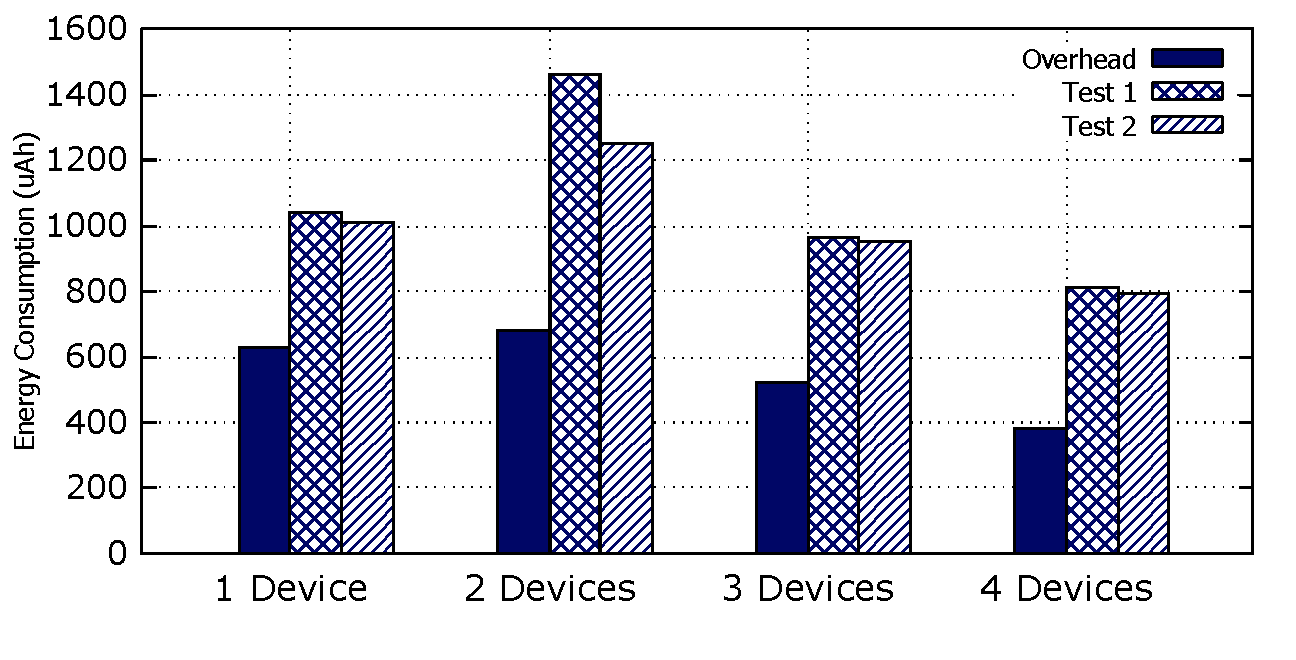
\includegraphics[width=0.45\textwidth]{data/img_energy.pdf}
	%}
	\caption{Performance and energy consumption of the large image processing tests in multiple clusters}
	\label{fig:cluster_performance}
\end{figure*}

\paragraph{Performance with large scale image}
Running the large scale image test case throughout 50 tests by increasing number of devices from 1 to 5 within the network, we found that the test case doesn't work if there is only one device standing desolately. By utilizing 2 threads for the image process on that single device, we realized that only 1 thread works, while the other does not, due to an out of memory exception, and the processing time to complete half of the task is $12,581ms$. 

By increasing the number of devices in network from 2 to 5 and sharing the task by sending jobs to other peers, we gathered average statistic data in 20 tests as in the Figure (\ref{fig:cluster_performance} - left) (clusters with 2, 3, 4 and more devices). In this Figure, to accomplish the task, the two devices have to work in $13,541ms$ average. The execution time reduced when more devices participate the cluster, down to average $7387ms$ when more than 4 peers joined the cluster, which is twice as fast as having 2 devices (notice that system didn't fully work with only one device).

To measure energy consumption on each device, we used Monsoon Power Monitor \cite{moosoon} and measured the velocity of energy drained on a single mobile device when utilizing power from the other peers. Figure \ref{fig:cluster_performance} (right) shows the energy measurement results from the two consecutive tests. Although the two tests showed the big gap when executing a 2 device cluster, in general the variability of energy consumption within multiple clusters matches with time consumption one. By running the two consecutive tests with the same input for 20 times, we realized that the results didn't change, and by utilizing 3 or more devices, we can significantly reduce the amount of energy required for the task, sometimes up to 25\%. However when we increased the number of devices in cluster, we didn't get the performance raised up at the corresponding value linearly, this can be explained by Amdahl's law \cite{amdahl}. Throughout our experiments, the number of devices at 3 to 5 will give the maximum benefit in terms of energy saving and device usage productivity.

\paragraph{Performance with normal scale image}
To make any device in the network feasible for image processing, we reduced the input image size to $2500 \times 1405$. By reconfiguring the cluster from 1 to 4 devices and measure total execution time on the callers, we gathered performance data among them as shown in Figure \ref{fig:small_img_perf}. From our statistic data, the total time consumed by one device to run on itself is slightly fluctuated around $5400ms$ between multiple measurements, but if one more device joins the network the time consumed is decreased to $3500ms$ which is 35\% faster. When more devices (3 or 4) participate, performance will continuously increase although their finishing time largely varies. Specifically 4 devices will collaboratively execute twice as fast as one device, or 50\% faster according to our measurements.

\begin{figure*}
	\centering
	%\resizebox{0.45\textwidth}{!}{
		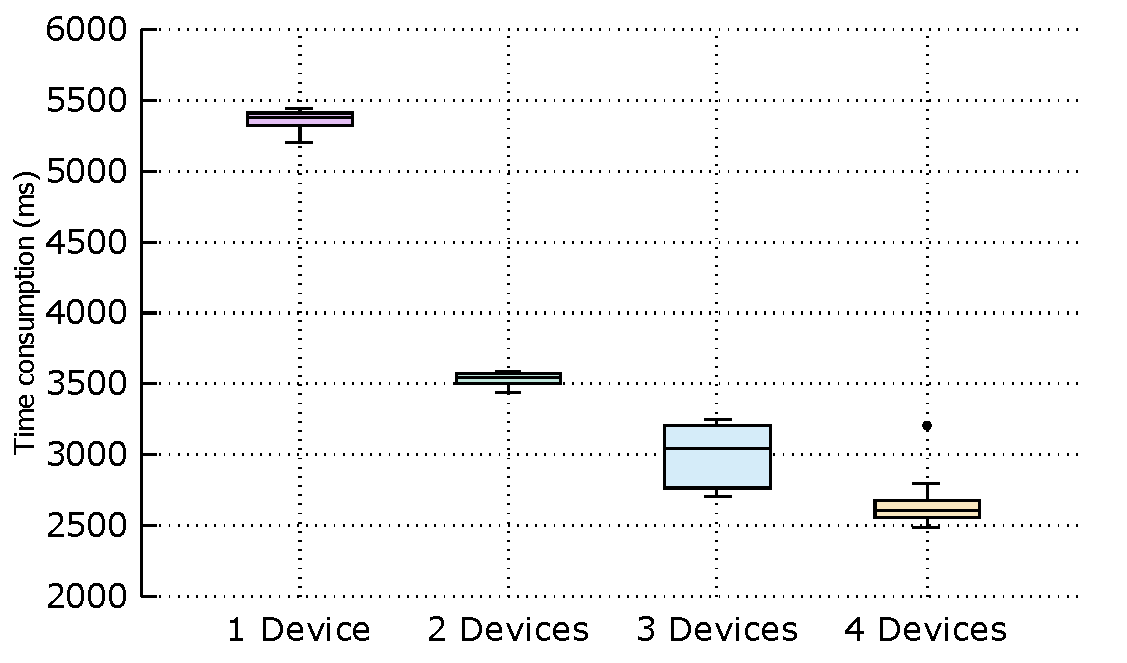
\includegraphics[width=0.48\textwidth]{data/img_small_perf_full.pdf}
		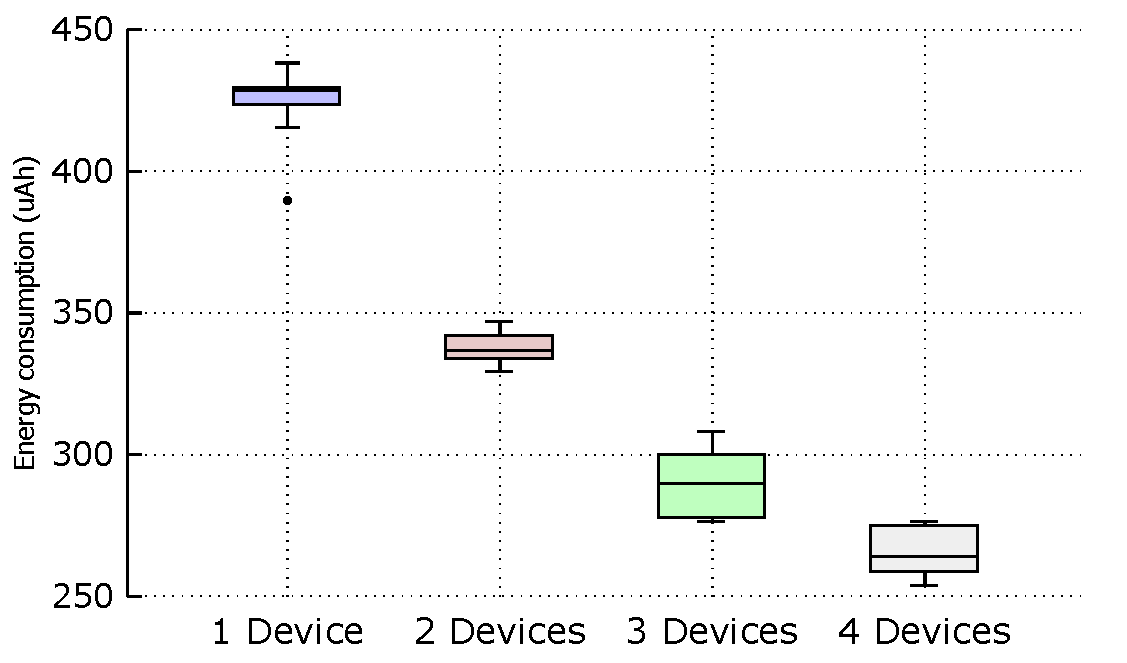
\includegraphics[width=0.45\textwidth]{data/img_small_energy.pdf}
	%}
	\caption{Performance and energy consumption of the image processing tests with a normal image size.}
	\label{fig:small_img_perf}
\end{figure*}

Basically the variability and fluctuation of energy consumption will reflect the performance, Figure (\ref{fig:small_img_perf} - right) displays the details. Through our experiments, running the cluster with 2 devices will preserve 20\% energy compare with 1 device, the number is better with 3 devices at $34\%$ and 4 devices at $37.5\%$ respectively.

%\begin{figure}
	%\centering
	%\resizebox{0.39\textwidth}{!}{
		%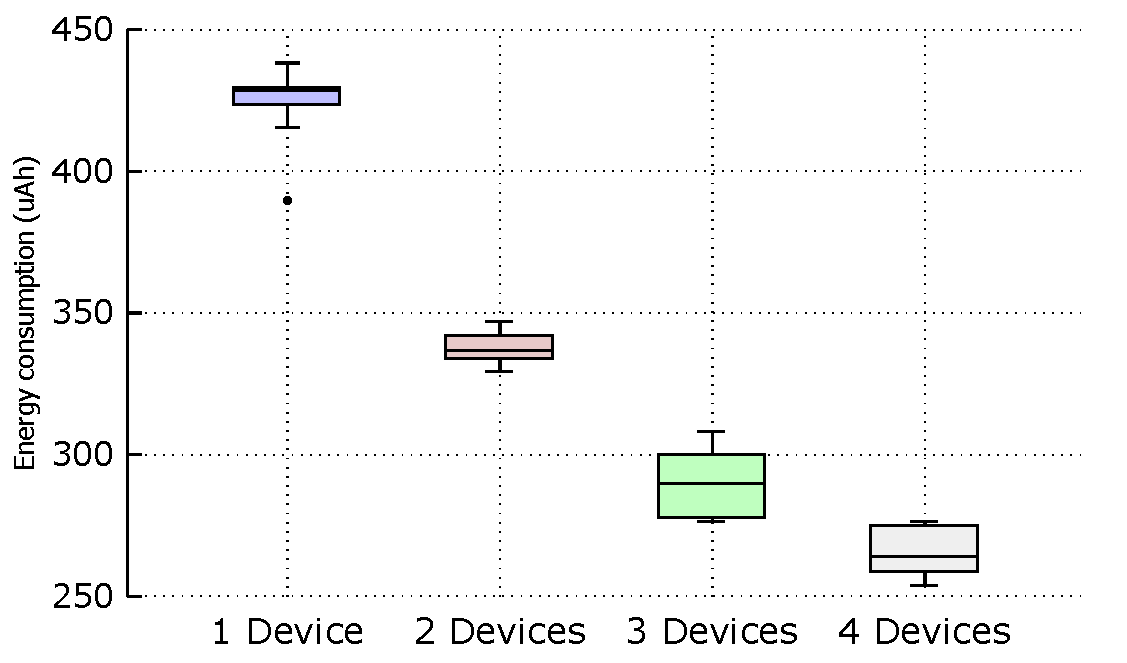
\includegraphics{data/img_small_energy.pdf}
	%}
	%\caption{Energy consumption from the image processing tests in multiple clusters.}
	%\label{fig:small_img_energy}
%\end{figure}

\subsubsection{Internet Access} 
Theoretically, remote accessibility won't help reducing the amount of bytes downloaded, however the speed is guaranteed to be ameliorative since the downloading process is scattered over a number of devices, therefore less energy will be consumed. 

\textbf{\emph{Design:}}
To apply APIs for this application, from the caller we dispatch job requests, which contain the information of job with resources including URL, number of parts and index, to the peers having \texttt{IRS[network]} at \texttt{high} or \texttt{low}. At each peer, when a request is received, it executes the job to load the URL to achieve a page in HTML code. Then it will parse the HTML to detect resource links including multimedia resources (images, audio, videos), CSS, and JS. Depending on the number of parts and index, it narrows down the amount of resources and attempt to download and put them into a ZIP file before throwing it back to the caller.

According to our system architecture, the caller needs to prepare a placeholder to hold every incoming result. For this test case, the placeholder is designated as a sub folder in the \texttt{Download} folder. When the result comes as a ZIP file, its contents will be extracted and filled into the placeholder folder. The final HTML file will contain all the modified resource links which are located at the same folder. Finally, the local HTML file can be opened by Android Web browser component using a local web server, for instance, TinyHTTPd \cite{tinyhttpd}.

\textbf{\emph{Performance:}}
Figure (\ref{fig:net_clusters_perf} - left) describes performance of multi-device clusters from 1 to more than 4 peers (some peers use a few more threads for simulating high performance) when remotely rendering web pages from CNN URLs. The figure describes the execution time of each peer in each cluster after being assigned a job, and the peak is reached when the last peer completes its work. In the cluster with only one device, it works desolately without any peer contacts; it will download web pages from the internet by opening Wi-Fi connection. It is obvious that executing Internet Remote access brings a high benefit in terms of performance since rendering time is reduced almost a half when at least 3 peers participate in the network. 

\begin{figure*}
	\centering
	%\resizebox{0.45\textwidth}{!}{
		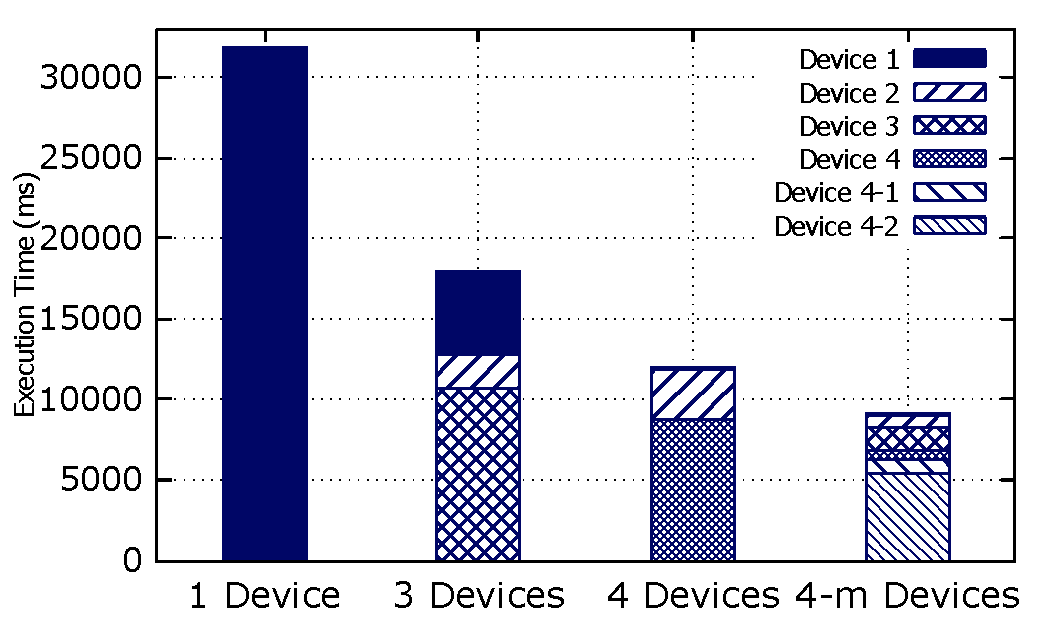
\includegraphics[width=.45\textwidth]{data/net_perf_01.pdf}
		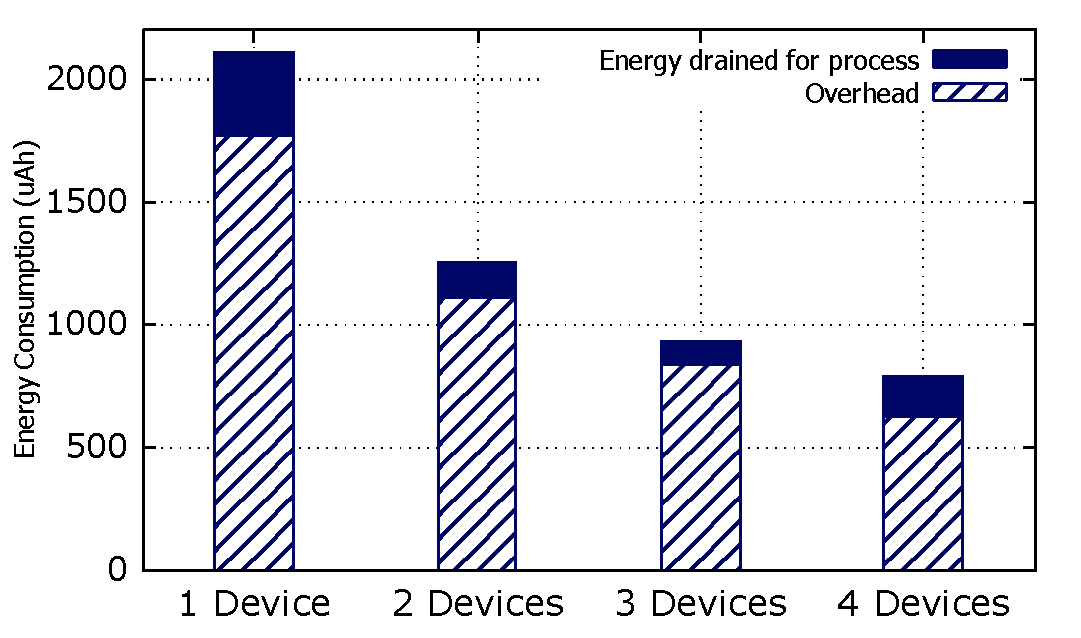
\includegraphics[width=.45\textwidth]{data/net_energy.pdf}
	%}
	\caption{Performance and energy consumption comparison for Internet sharing}
	\label{fig:net_clusters_perf}
\end{figure*}

To evaluate energy consumption, we performed the same tests similar to the first test case by measuring in multi-device clusters with overheads and when remotely rendering web pages. From the outcome of energy test (Figure \ref{fig:net_clusters_perf} - right), we realized that by handing over computation utilizing system resources (Here is Internet accessibility) over peer-to-peer network with multiple peers will help reducing significantly energy consumed, particularly more than a half in compare with a solo device. The differences between the total energy and overheads are not fluctuated much between the multiple clusters, which can be easily explained by \cite{wifi_energy}.\\

%\begin{figure}
	%\centering
	%\resizebox{0.39\textwidth}{!}{
		%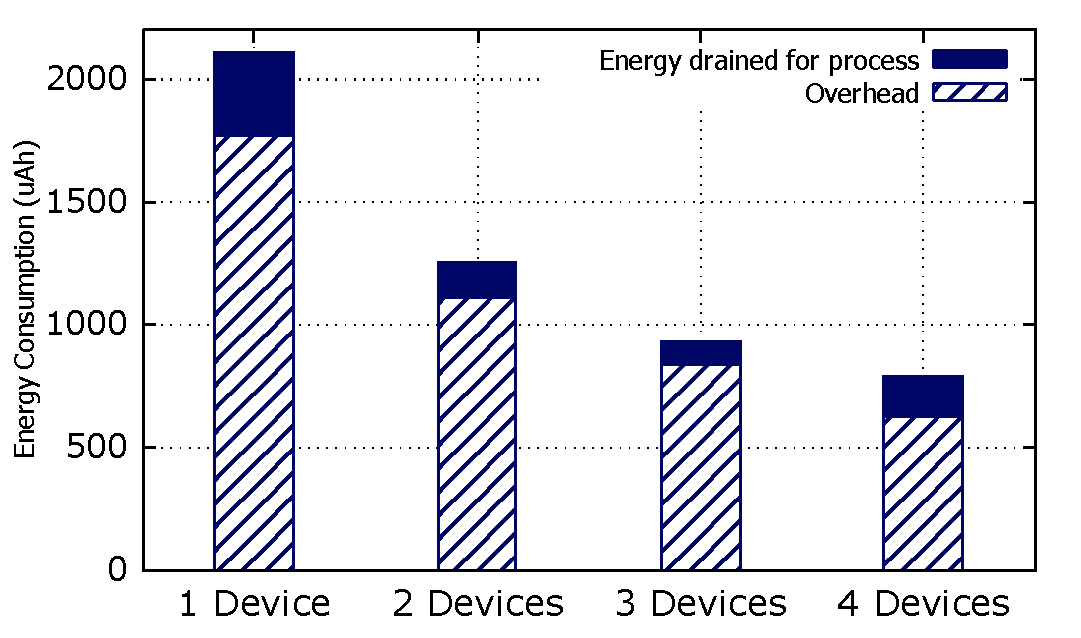
\includegraphics{data/net_energy.pdf}
	%}
	%\caption{Energy consumption of clusters for Internet sharing}
	%\label{fig:net_cluster_energy}
%\end{figure}

\subsubsection{GPS Share}
Connecting and retrieving the GPS location is really energy consuming. Generally the smartphone will enable and contact at least 3 satellites through radio signals in order to start retrieving the GPS location (4 satellites to get more information like altitude). Therefore, energy can be saved if GPS requests are relayed to another device in the network which is healthier (higher remaining battery, in idle state, etc.) or has better specifications.

\textbf{\emph{Design}}
With GPS Share, only one peer is entrusted. Our strategy is letting the caller to select the peer having GPS enabled and maximum value of $RL$ (at the best condition) by configuring the caller with initiative criteria including $RL$ is \texttt{max} and \texttt{GPS} is \texttt{on}. Regarding job definition, we utilize the \texttt{LocationManager} to get a single location result per each request and store the result to a simple string. For remote GPS request, we have to avoid callback functions from \texttt{LocationManager}; therefore, retrieving multiple requests periodically is not effective.


\textbf{\emph{Performance}}
We performed 3 GPS Share test cases, 2 for remote GPS requests and 1 for local GPS (Using GPS on it own). For each case we execute $10$ times on two devices with the same specifications and assign roles to them as a caller and a receiver to minimize the overloads throughout the system. Figure \ref{fig:gps_perf} interprets that GPS Share mechanism doesn't give any benefit in terms of performance, since the remote device has the same resource specs and remote GPS may require even more time including time for GPS plus time for data transmission back to the caller (however it is too short for consideration).

\begin{figure*}
	\centering
	%\resizebox{0.36\textwidth}{!}{
		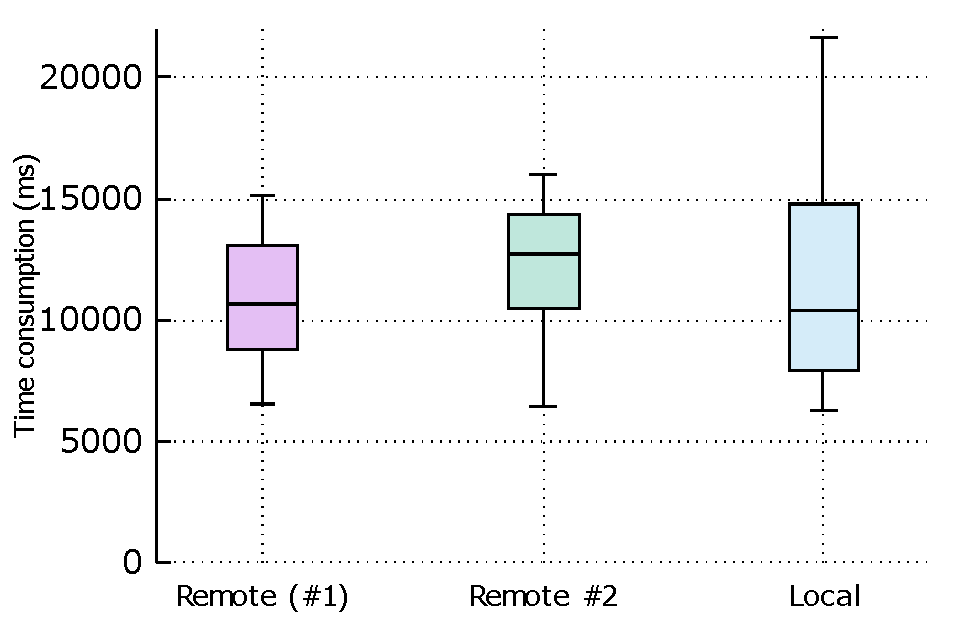
\includegraphics[width=.42\textwidth]{data/gps_perf.pdf}
		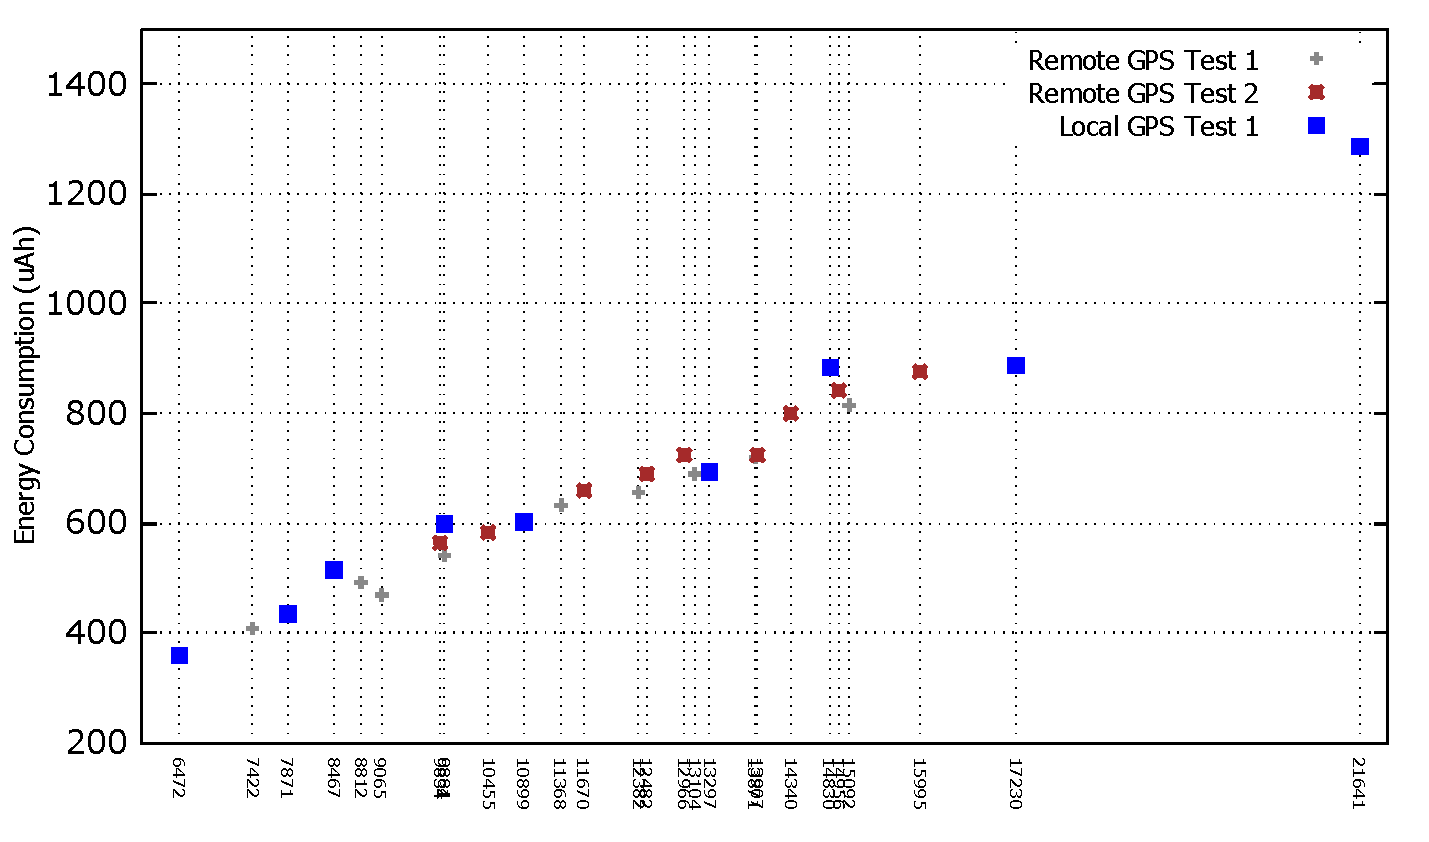
\includegraphics[width=.47\textwidth]{data/gps_energy_full.pdf}
	%}
	\caption{Performance and energy consumption comparison between remote and local GPS sensing.}
	\label{fig:gps_perf}
\end{figure*}

Extracted from the above tests, Figure \ref{fig:gps_perf} describes the distribution of energy consumptions among the 3 test cases. By applying interpolation to find trend lines for these energy distributions, we got $y = 0.0528388 \times x + 7.31948$ formula for test 1, $y = 0.0547221 \times x + 7.42138$ for test 2 and $y = 0.0575331 \times x - 12.9403$ for test 3. The trend line 3 has the biggest slope, or at the same amount of time it consumed more energy than the first two cases. As we might see, the difference between the slopes of line 3 and line 1, 2 are very slim, however due to our later tests on the weak caller (low battery), the difference will highly increase. 

\textbf{\emph{Applications}}
By integrating our system with either RetroSkeleton \cite{retro-skel} or Rio \cite{rio}, we can provide remote or local GPS location data without having to modify the current installed applications. Those systems provide interference methods to capture requests for system resources and instead inject their customized responses. 

\section{Related Work}
\label{sec:related}
The work presented here is related to other complementary efforts that optimize mobile applications via remote executions including computation offloading and peer to peer networking.

Alljoyn \cite{alljoyn} is an open source framework that hides the complexity of network communications for application programmers. By providing interoperability between multiple platforms without any transport layers, Alljoyn makes the integration and initiation of network communication easy and simple. 

Before the Wi-Fi Direct available in software industry, many efforts to address P2P networks, Frank H. P. Fitzek et al. \cite{m_p2p_tutor} summarized the relevant papers focusing on this topic to demonstrate the initiative steps to establish the point-to-point collaborative Wi-Fi networks. Liam McNamara et al. published \cite{media_share} media sharing based on historical colocation information over urban transport using blue-tooth or any available wireless connections.

Since the modern mobile devices (phones and tablets) are featured with multiple network capabilities, many researches relied on these features to exchange resources and computations. Ardalan et al. designed Rio \cite{rio} bases on I/O device files to share contents and resources among the applications in different devices without having to modify them. Their use-cases addressed multi-system photography and gaming, singular SIM card for multi-devices, music and video sharing. Nairan Zhang et al. developed GameOn \cite{gameon} to utilize Wi-Fi P2P to establish non-Internet connection between the gamers, which majorly focuses on closed range network like in public transportation, bus or train. The other content sharing systems CAMEO \cite{cameo}, Spartacus \cite{spartacus} and GigaSight \cite{crowd-sourcing} try to detect closed range networks base on specific methods to distributed data. Utilizing Doppler effect applying on built-in microphones and speakers, Spartacus help can initiate and interact with nearby devices through pointing gesture with accuracy up to 90\% within distance of 3 meters.

In terms of improving energy consumption, offloading-featured systems like MAUI \cite{maui}, COMET \cite{comet}, \cite{kwon+:mobilesoft15}, \cite{mobile-cloud-middleware} or \cite{fuzzy-engine} address the heavy computations by offloading source code or execution module to server following multiple constraints and policies to release workload and energy consumed at client which is either mobile device or low computation capacity computer. 

\section{Conclusions}
\label{sec:conc}
%Our future research direction will 
%
In this paper, we have presented an extended distribution framework to increase quality of service in resources-limited execution environments. Our approach improves the energy efficiency and performance of mobile applications with a simple programming model and a novel runtime system by leveraging either cloud infrastructures or nearby mobile devices. In addition, our approach can bring a new hardware feature to the existing mobile devices. We have evaluated our approach by reducing the execution time and the energy consumption of case study applications as well as enabling a mobile device to utilize a GPS sensor from nearby mobile devices. These results indicate that our approach represents a promising direction in developing complex mobile applications for resource-limited mobile devices.

%\section*{Acknowledgment}
%This research is supported by Utah State University through the RC Grant.

\balance
\bibliographystyle{abbrv}
\bibliography{references}

\end{document}

